\documentclass[12pt]{article}
\usepackage{amsmath}
\usepackage{geometry}
\usepackage{graphicx}
\usepackage{hyperref}
\usepackage[latin1]{inputenc}
\usepackage{listings}
\renewcommand{\labelitemi}{$\textendash$}
\geometry{
    a4paper,
    total={170mm,257mm},
    left=15mm,
    right=15mm,
    top=5mm,
    bottom=15mm
}

\title{CS4061: Week 2 Assignment}
\author{Conor McCauley - 17323203}
\date{October 20, 2020}

\begin{document}

\maketitle

\noindent \textbf{Dataset Identifier:} \texttt{\# id:18--18-18 }

\section*{Question (a)}

\noindent (i) The below plot shows the values from the dataset. The first feature, $x_1$, is plotted along the x-axis while the second feature, $x_2$, is plotted along the y-axis. Target values of $+1$ are represented as green dots while target values of $-1$ are represented as blue dots:

\begin{center}
    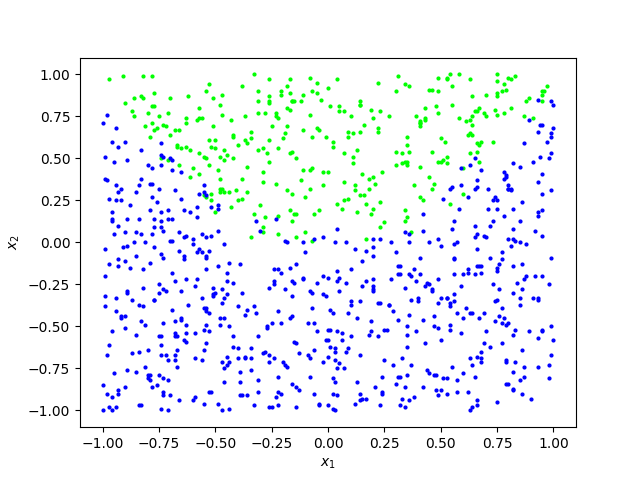
\includegraphics[scale=0.6]{fig_1.png}
\end{center}

\noindent (ii) The \texttt{part\_a\_ii()} method in the code uses SciKit's \texttt{LogisticRegression} to train a logistic regression classifier on the downloaded dataset. Both features, $x_1$ and $x_2$, can be combined into a single array using Numpy: \texttt{np.column\_stack((X1, X2))} - this array can be used as our training data (alongside an array of the target values):

\begin{center}
    \lstset{basicstyle=\footnotesize}
    \begin{lstlisting}[language=Python]
    X1 = np.array(filter_data(data, 0)).reshape(-1, 1)
    X2 = np.array(filter_data(data, 1)).reshape(-1, 1)
    X = np.column_stack((X1, X2))
    Y = np.array(filter_data(data, 2))
    model = LogisticRegression(penalty='none', solver='lbfgs').fit(X, Y)
    \end{lstlisting}
\end{center}

The trained model produced the following parameter values which we will use to determine the boundary function in the next question:

\begin{center}
    \begin{tabular}{|c|c|c|}
        \hline
        $\theta_0$ & $\theta_1$ & $\theta_2$ \\
        \hline
        $-2.233$ & $-0.253$ & $6.543$ \\
        \hline
    \end{tabular}
\end{center}

\noindent (iii) The \texttt{part\_a\_iii()} method in the code uses the model's \texttt{predict()} function to predict target values for each of the input features using our trained model from part (ii):

\begin{center}
    \lstset{basicstyle=\footnotesize}
    \begin{lstlisting}[language=Python]
    X = np.column_stack((X1, X2))
    Y = np.array(filter_data(data, 2))
    predictions = model.predict(X)
    \end{lstlisting}
\end{center}

In order to determine the decision boundary we need to solve our new feature equation in terms of $y$ (i.e., $x_2$) so that we have an equation of a line. We do this by finding both the axis intercepts and then calculating the slope, etc.:

$$\theta_1x + \theta_2y + \theta_0 = 0$$

$$x = -\frac{\theta_2y + \theta_0}{\theta_1}, y = 0 \implies x = -\frac{\theta_0}{\theta_1}$$

$$y = -\frac{\theta_1x + \theta_0}{\theta_2}, x = 0 \implies y = -\frac{\theta_0}{\theta_2}$$

$$y = -\frac{\theta_1x + \theta_0}{\theta_2}$$

The below plot shows the dataset's training values, the model's predicted values and the decision boundary. Orange dots represent incorrectly predicted $+1$ values while black dots represent incorrectly predicted $-1$ values, green and blue dots represent correctly predicted $+1$ and $-1$ values, respectively:

\begin{center}
    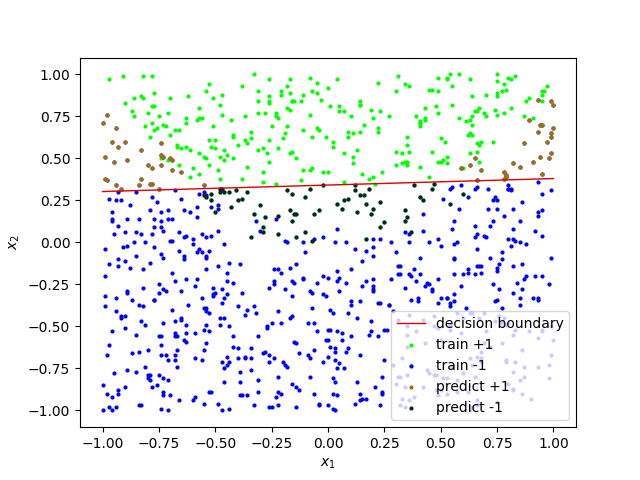
\includegraphics[scale=0.8]{fig_2.png}
\end{center}

\noindent (iv) As could be seen in the original plot the target values seem to be split by some type of quadratic curve. As such, a logistic regression model - which \textbf{in this case} uses a linear equation derived from two features to predict target values - would always incorrectly predict target values for a not insignificant number of inputs. However, using SciKit's \texttt{accuracy\_score()} method we can see that the trained model correctly predicts the target values for $87.6\%$ of the inputs:

\begin{center}
    \lstset{basicstyle=\footnotesize}
    \begin{lstlisting}[language=Python]
    predictions = model.predict(X)
    accuracy = accuracy_score(Y, predictions)
    print('accuracy = %f' % (accuracy))
    \end{lstlisting}
\end{center}

For reference, a baseline model, which always predicted the most common target value ($-1$) would make correct predictions $67.3\%$ of the time. Our trained model is significantly more accurate than the baseline model - which is to be expected.

\section*{Question (b)}

\noindent (i) Using SciKit's \texttt{LinearSVC()} method we can train linear SVM classifiers on our dataset for a number of different penalty parameters, $C$:

\begin{center}
    \lstset{basicstyle=\footnotesize}
    \begin{lstlisting}[language=Python]
    X = np.column_stack((X1, X2))
    Y = np.array(filter_data(data, 2))
    for C in (0.001, 1, 1000):
        model = LinearSVC(C=C).fit(X, Y)
        predictions = model.predict(X)
    \end{lstlisting}
\end{center}
As the code to do this is practically identical to the code from (a) I will not add any additional explanations here. It produces the following parameter values:

\begin{center}
    \begin{tabular}{|c|c|c|c|}
        \hline
        $C$ & $\theta_0$ & $\theta_1$ & $\theta_2$ \\
        \hline
        $0.001$ & $-0.228$ & $0.001$ & $0.484$ \\
        $1$ & $-0.709$ & $-0.076$ & $2.097$ \\
        $1000$ & $-1.597$ & $-0.886$ & $3.625$ \\
        \hline
    \end{tabular}
\end{center}

\noindent (ii) As in (a), we can use the SVM's \texttt{predict()} function to predict target values for each of the input features using each of our trained models from (i). We can also calculate the decision boundaries for each of the models using the same 'equation of a line' method from (a). The below plots show the training values, the predicted values and the decision boundaries for different values of $C$:

\begin{center}
    
    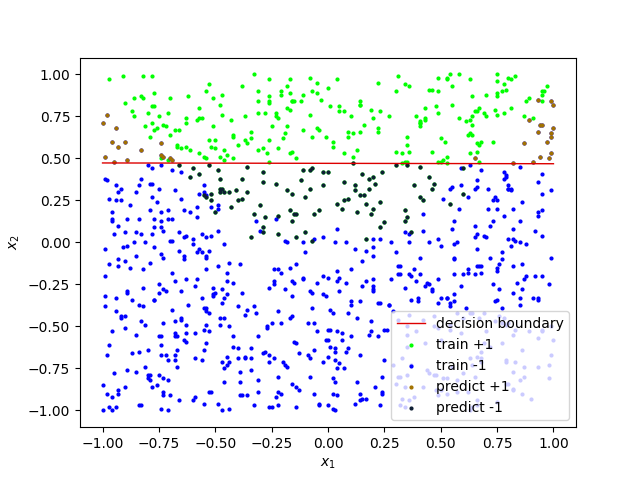
\includegraphics[scale=0.7]{fig_3.png}
    
    $C = 0.001$
    
    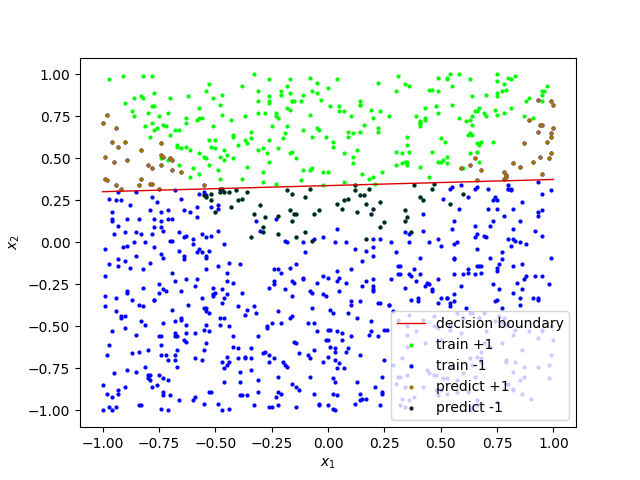
\includegraphics[scale=0.7]{fig_4.png}
    
    $C = 1$
    
    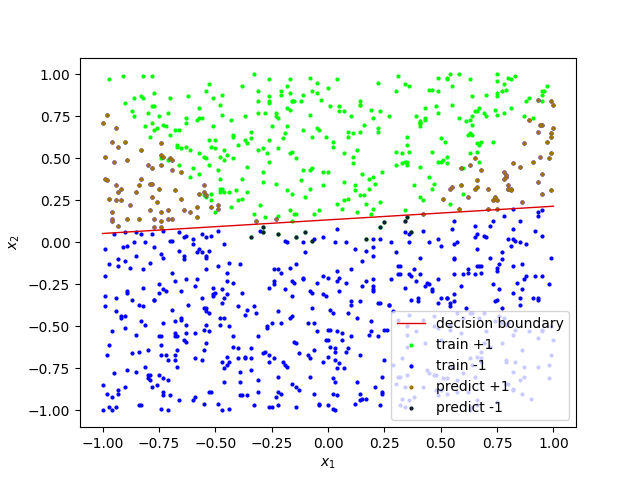
\includegraphics[scale=0.7]{fig_5.png}
    
    $C = 1000$
    
\end{center}

\noindent (iii) Again, using SciKit's \texttt{accuracy\_score()} method we can determine the predictive accuracy of each of the models:

\begin{center}
    \begin{tabular}{|c|c|}
        \hline
        $C$ & Accuracy \\
        \hline
        $0.001$ & $87.17\%$ \\
        $1$ & $87.77\%$ \\
        $1000$ & $82.16\%$ \\
        \hline
    \end{tabular}
\end{center}

Increasing the penalty parameter, $C$, increases the absolute values of each of the parameter values. For $C = 1000$ the SVM does not converge on an accurate result in the default number of iterations (SciKit even warns of this in the console). For $C = 0.001$ the iterative changes in the parameter values are a bit too small to converge on the 'correct' result in the default number of iterations. However, for $C = 1$, the SVM produces predictions that are even more accurate than our logistic regression classifier from (a). Increasing $C$ decreases the effect a large cost will have on each successive iteration. As such, if $C$ is too large then the number of iterations that are required to minimise the cost function. Conversely, if $C$ is too small then we may 'over-shoot' in each iteration by over-penalising high costs. From the above result it would seem that a penalty parameter of $C = 1$ was the optimum middle-ground for this model.

\section*{Question (c)}

\noindent (i) We can create the two new features, $x_3$ and $x_4$, such that $x_3$ contains the squares of each element in $x_1$ and $x_4$ contains the squares of each element in $x_2$. We can then train a logistic regression classifier using the same method we used in (a):

\begin{center}
    \lstset{basicstyle=\footnotesize}
    \begin{lstlisting}[language=Python]
    X = np.column_stack((X1, X2, X3, X4))
    Y = np.array(filter_data(data, 2))
    model = LogisticRegression(penalty='none', solver='lbfgs').fit(X, Y)
    \end{lstlisting}
\end{center}

The model reports the following five parameter values which can be used in (iv) to determine the boundary function:

\begin{center}
    \begin{tabular}{|c|c|c|c|c|}
        \hline
        $\theta_0$ & $\theta_1$ & $\theta_2$ & $\theta_3$ & $\theta_4$\\
        \hline
        $-0.132$ & $-0.414$ & $21.236$ & $-23.759$ & $6.031$ \\
        \hline
    \end{tabular}
\end{center}

\noindent (ii) As in the previous questions, we can use SciKit's \texttt{predict()} function to predict target values for each input. Plotting these predictions produces the following graph:

\begin{center}
    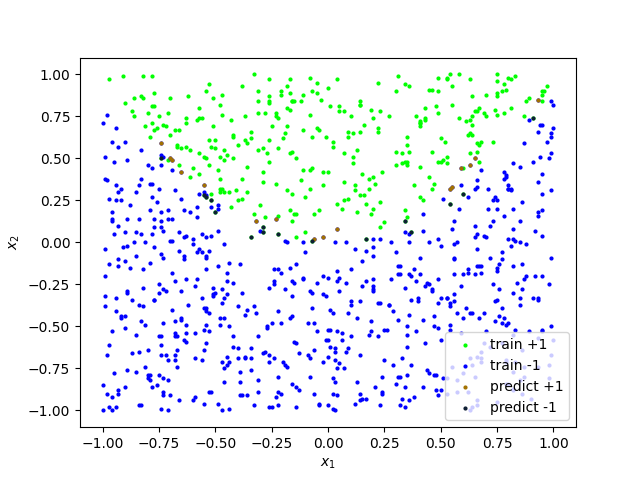
\includegraphics[scale=0.8]{fig_6.png}
\end{center}

It is evident from this plot that the addition of the two new features allowed the model to more accurately predict the target values - the reported accuracy was $96.8\%$. In fact, the incorrectly predicted values may just be the result of noise and increasing the number of features any further might lead to overfitting.

\noindent (iii) As mentioned in a previous question, a baseline predictor which always predicted the most common target value ($-1$) would be correct $67.3\%$ of the time. Our model, which is correct $96.8\%$ of the time, represents a very significant improvement over the baseline model.

\noindent (iv) In order to plot the decision boundary we must rewrite the equation of our features in terms of $y$ (i.e., $x_2$). Seeing as we added the squares of $x$ ($x_1$) and $y$ ($x_2$) as features we can assume that the equation is of the following form:

$$\theta_0 + \theta_1x + \theta_2y + \theta_3x^2 + \theta_4y^2 = 0$$

This is clearly a quadratic equation, which we can solve as follows:

$$\theta_4y^2 + \theta_2y + (\theta_3x^2 + \theta_1x + \theta_0) = 0$$

$$y = \frac{-\theta_2 \pm \sqrt{\theta_2^2 - 4\theta_4(\theta_3x^2 + \theta_1x + \theta_0)}}{2\theta_4}$$

Adding this line to our previous plot produces the following graph:

\begin{center}
    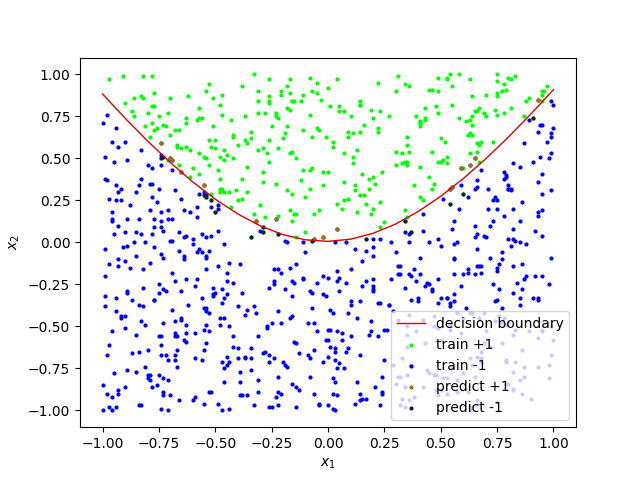
\includegraphics[scale=0.8]{fig_7.png}
\end{center}

\section*{Appendix: Code}

\lstset{basicstyle=\footnotesize}
\begin{lstlisting}[language=Python]
from sklearn.linear_model import LogisticRegression
from sklearn.metrics import accuracy_score
from sklearn.svm import LinearSVC
import matplotlib.pyplot as plt
import numpy as np
import pandas as pd

# select specific feature from the data with an optional target value filter
def filter_data(data, index, filter=None):
    if filter: return [d[index] for d in data if d[2] == filter]
    else: return [d[index] for d in data]

# plot the training data as well as a model's predicted results
# `boundary_f` is a lambda function for calculating the decision boundary
def plot_training_data_and_predictions(data, predictions, boundary_f=None):
    # plot training data
    X1, Y1 = filter_data(data, 0, filter=1), filter_data(data, 1, filter=1)
    X2, Y2 = filter_data(data, 0, filter=-1), filter_data(data, 1, filter=-1)
    plt.scatter(X1, Y1, marker='o', c='#00ff00', s=4)
    plt.scatter(X2, Y2, marker='o', c='#0000ff', s=4)
    # plot only the incorrect predictions instead of replotting everything
    X1, Y1 = [], []
    X2, Y2 = [], []
    for i, target in enumerate(predictions):
        if target == 1 and data[i][2] != 1:
            X1.append(data[i][0])
            Y1.append(data[i][1])
        elif target == -1 and data[i][2] != -1:
            X2.append(data[i][0])
            Y2.append(data[i][1])
    plt.scatter(X1, Y1, marker='o', c='#a37200', s=4)
    plt.scatter(X2, Y2, marker='o', c='#0e1e33', s=4)
    # calculate and plot decision boundary
    if boundary_f:
        X = np.arange(-1, 1.1, 0.1)
        plt.plot(X, boundary_f(X), c='#dd0000', linewidth=1)
    # show plot
    plt.xlabel('$x_1$')
    plt.ylabel('$x_2$')
    if boundary_f:
        plt.legend(['decision boundary', 'train +1', 'train -1',
            'predict +1', 'predict -1'])
    else:
        plt.legend(['train +1', 'train -1',
            'predict +1', 'predict -1'])
    plt.show()
    return

def part_a_i(data):
    X1, Y1 = filter_data(data, 0, filter=1), filter_data(data, 1, filter=1)
    X2, Y2 = filter_data(data, 0, filter=-1), filter_data(data, 1, filter=-1)
    plt.scatter(X1, Y1, marker='o', c='#00ff00', s=4)
    plt.scatter(X2, Y2, marker='o', c='#0000ff', s=4)
    plt.xlabel('$x_1$')
    plt.ylabel('$x_2$')
    plt.show()

def part_a_ii(data):
    X1 = np.array(filter_data(data, 0)).reshape(-1, 1)
    X2 = np.array(filter_data(data, 1)).reshape(-1, 1)
    X = np.column_stack((X1, X2))
    Y = np.array(filter_data(data, 2))
    model = LogisticRegression(penalty='none', solver='lbfgs').fit(X, Y)
    print('intercept = %f, slopes = (%f, %f)' %
        (model.intercept_, *model.coef_[0]))
    return model

def part_a_iii(data, model):
    # use trained model to predict target values
    X1 = np.array(filter_data(data, 0)).reshape(-1, 1)
    X2 = np.array(filter_data(data, 1)).reshape(-1, 1)
    X = np.column_stack((X1, X2))
    Y = np.array(filter_data(data, 2))
    predictions = model.predict(X)
    accuracy = accuracy_score(Y, predictions)
    print('accuracy = %f' % (accuracy))
    # set up decision boundary function
    m0, m1, c = model.coef_[0][0], model.coef_[0][1], model.intercept_
    boundary_f = lambda x: -((m0 * x) + c) / m1
    # plot everything
    plot_training_data_and_predictions(data, list(predictions), boundary_f)

def part_a(data):
    part_a_i(data)
    model = part_a_ii(data)
    part_a_iii(data, model)

def part_b(data):
    X1 = np.array(filter_data(data, 0)).reshape(-1, 1)
    X2 = np.array(filter_data(data, 1)).reshape(-1, 1)
    X = np.column_stack((X1, X2))
    Y = np.array(filter_data(data, 2))
    for C in (0.001, 1, 1000):
        # train model and predict target values
        model = LinearSVC(C=C).fit(X, Y)
        predictions = model.predict(X)
        accuracy = accuracy_score(Y, predictions)
        print('C = %f >> intercept = %f, slopes = (%f, %f) >> accuracy = %f' %
            (C, model.intercept_, *model.coef_[0], accuracy))
        # set up decision boundary function
        m0, m1, c = model.coef_[0][0], model.coef_[0][1], model.intercept_
        boundary_f = lambda x: -((m0 * x) / m1 + (c / m1))
        # plot everything
        plot_training_data_and_predictions(data, list(predictions), boundary_f)

def part_c(data):
    # add new features
    X1, X2, X3, X4 = [], [], [], []
    for x1, x2, _ in data:
        X1.append(x1)
        X2.append(x2)
        X3.append(pow(x1, 2))
        X4.append(pow(x2, 2))
    # train a model and predict target values
    X1 = np.array(X1).reshape(-1, 1)
    X2 = np.array(X2).reshape(-1, 1)
    X3 = np.array(X3).reshape(-1, 1)
    X4 = np.array(X4).reshape(-1, 1)
    X = np.column_stack((X1, X2, X3, X4))
    Y = np.array(filter_data(data, 2))
    model = LogisticRegression(penalty='none', solver='lbfgs').fit(X, Y)
    print('intercept = %f, slopes = (%f, %f, %f, %f)' %
        (model.intercept_, *model.coef_[0]))
    predictions = model.predict(X)
    accuracy = accuracy_score(Y, predictions)
    print('accuracy = %f' % (accuracy))
    # set up decision boundary function
    m0, m1, m2, m3 = model.coef_[0]
    c = model.intercept_
    boundary_f = lambda x: (-m1 + pow(m1*m1 - 4*m3*(m2*x*x + m0*x + c), 0.5)) / 2*m3
    # plot everything
    plot_training_data_and_predictions(data, list(predictions), boundary_f)

data = pd.read_csv('dataset.csv', comment='#').values.tolist()
part_a(data)
part_b(data)
part_c(data)
\end{lstlisting}

\end{document}
